\chapter{Evaluation und Ergebnisse}
\label{chap:benchmark}
In diesem Kapitel wird ein Benchmark durchgeführt, der die Performance des Executors in Bezug auf die Laufzeit den nativen Frameworks gegenüberstellt. Verglichen wird dabei die benötigte Zeit für die Erstellung, die Ausführung sowie die Gradientenberechnung der Quantenschaltkreise. Zunächst wird der experimentelle Aufbau der Messungen detailliert beschrieben. Anschließend werden die Ergebnisse anhand von Diagrammen visuell aufbereitet und diskutiert. Ziel dieser Untersuchung ist es, die Laufzeiteffizienz des Executors zu bestimmen und den zeitlichen Overhead gegenüber der direkten Nutzung der nativen Frameworks zu quantifizieren.

\section{Aufbau der Messung}
\label{sec:benchmark-aufbau}

Gemessen wird nicht die Leistung der Simulatoren selbst, sondern der Aufwand, den
die Abstraktionsschicht zusätzlich verursacht. Da im Messfenster jeweils der
gesamte Aufruf einschließlich der Simulation liegt, lässt sich dieser Aufwand nur
über einen Vergleich bestimmen. Jede Messung wurde deshalb zweimal durchgeführt,
einmal direkt über die native API des Frameworks und einmal über den Executor mit
demselben Framework als Backend. Die erste Variante wird im Folgenden als
nativer Benchmark bezeichnet. Da beide Seiten denselben Simulator mit demselben
Schaltkreis aufrufen, kürzt sich der Simulationsanteil im Verhältnis der beiden
Laufzeiten weitgehend heraus. Dieses Verhältnis wird als Overhead-Faktor angegeben.

Damit wirklich derselbe Schaltkreis ausgeführt wird, entsteht die Gattersequenz
zunächst framework-unabhängig aus einem festen Seed und wird erst danach in beide
Darstellungen übersetzt. Genutzt wurde ein Set aus 13 Clifford- und
Nicht-Clifford-Gattern. Die Gatterzahl läuft über 20 logarithmisch verteilte Werte
zwischen 10 und 100\,000, die Qubit-Zahl über 5, 8, 10 und 12. Jede Zelle wurde
viermal mit unterschiedlichen Zufallsschaltkreisen gleicher Größe wiederholt.

Als Messgröße dient die Wall-Clock-Zeit über \texttt{time.perf\_counter()}. Vor
jeder Messung läuft ein ungemessener Aufruf, damit Lazy-Imports und interne Caches
nicht in die Messung fallen. Im Messfenster liegt ausschließlich der jeweils
untersuchte Aufruf, während die Erzeugung des Devices, der Aufbau des Circuits und
die Instanziierung des Estimators zur ungemessenen Setup-Phase gehören.

Gemessen wurde in drei Modi, die typische Phasen eines variationellen Workflows
abbilden. Der Modus \texttt{creation} baut nur die Circuit-Repräsentation des jeweiligen Frameworks oder Executors auf, der
Modus \texttt{execution} wertet den Erwartungswert $\expval{Z_0}$ aus und der Modus
\texttt{gradient} bildet dessen analytische Ableitung. Für den Gradienten wurde
jedes dritte Gatter durch eine trainierbare Rotation ersetzt, sodass die Gatterzahl
konstant bleibt, während die Zahl der Ableitungsrichtungen mit
$n_{\mathrm{trainable}} = \lceil n_{\mathrm{gates}}/3 \rceil$ mitwächst.

\section{PennyLane und Executor im Vergleich}
\label{sec:vergleich-pennylane}
Für den Vergleich wird die native \textit{PennyLane}-QNode dem Executor auf dem
\textit{PennyLane}-Backend gegenübergestellt. Das Ergebnis ist auf beiden Seiten
dasselbe, nur der Weg dorthin unterscheidet sich. Die native Implementierung spricht
\textit{PennyLane} unmittelbar an, der Executor dagegen erst über die abstrakte
Zwischenschicht. Was an Zeit zwischen beiden liegt, geht damit auf die Abstraktion
zurück.

Alle übrigen Bedingungen wurden konstant gehalten. Als Simulator dient in beiden
Fällen \texttt{qml.\allowbreak device(\textquotedbl default.\allowbreak qubit\textquotedbl)} im analytischen Modus mit
\texttt{shots=None}, wobei die native Implementierung die Wire-Zahl vorgibt und der Executor sie
offen lässt. Ein Ergebnis-Cache kommt weder bei der QNode über \texttt{cache=False}
noch beim Executor über den Standardwert \texttt{caching=False} zum Einsatz. Die
Gattersequenz stammt aus demselben Generator mit demselben Seed, sodass jeweils
derselbe Schaltkreis entsteht. Auch die Observable stimmt überein, denn der Executor
übersetzt \texttt{Abstract\allowbreak Quantum\allowbreak Operator\allowbreak(paulis=[\textquotedbl I...IZ\textquotedbl], \allowbreak coeffs=\allowbreak[1.0])} nach \texttt{qml.\allowbreak expval\allowbreak(1.0 \allowbreak * \allowbreak Z(0))} und damit bis auf den skalaren Faktor nach
\texttt{qml.\allowbreak expval(qml.\allowbreak PauliZ(0))}. Der Messablauf ist ebenfalls identisch, mit vier
Wiederholungen, einem frischen Schaltkreis je Wiederholung und einem ungemessenen
Warm-up-Aufruf vorab. Der Aufbau von Gerät, QNode und Executor bleibt auf beiden
Seiten außerhalb des Messfensters.

Dadurch fällt in jedem der drei Modi auf beiden Seiten dieselbe Arbeit an, und die
Differenz spiegelt allein den Aufwand der Abstraktion wider. Was das im Einzelnen
bedeutet, zeigen die folgenden Absätze.

\paragraph*{Modus \texttt{creation}}\mbox{}\\
Die native Implementierung misst \texttt{qml.\allowbreak workflow.\allowbreak construct\_tape\allowbreak(circuit)()}. Dieser Aufruf
läuft einmal durch die Quantenfunktion und trägt sämtliche Operationen in ein
\texttt{QuantumTape} ein, ohne das Gerät anzusprechen oder zu simulieren.

Beim Executor wird \texttt{ex.\allowbreak transpile\_circuit\allowbreak(build\_abstract\allowbreak(...))} gemessen.
Zunächst entsteht die abstrakte Gatterliste, anschließend deren Übersetzung ins
native Format, also Listen aus \textit{PennyLane}-Operationen, Wires und Winkeln.
Auch hier bleibt es beim reinen Aufbau ohne Tape und ohne Simulation, weshalb die
Differenz ausschließlich aus dem Erstellen und Übersetzen der Gatterliste besteht.

\paragraph*{Modus \texttt{execution}}\mbox{}\\
Die native Implementierung misst \texttt{circuit()}. Der Aufruf zeichnet die Quantenfunktion auf,
reicht das Tape an das Preprocessing des Geräts weiter, simuliert und liefert
$\expval{Z_0}$.

Beim Executor wird \texttt{ex.\allowbreak expectation\_value\allowbreak(qc\_abs, \allowbreak op)} gemessen, wobei
Schaltkreis und Observable zu diesem Zeitpunkt bereits vorliegen. Ins Messfenster
fallen die Normalisierung der Parameter, der Cache-Lookup des Circuits, der Aufbau
einer neuen QNode sowie die Simulation. Für den Lookup wird
\texttt{hash\allowbreak(AbstractQuantumCircuit)} gebildet, was über sämtliche Gatter läuft. Neu
eingereiht werden die Operationen bei jedem Aufruf ohnehin auf beiden Seiten, auf
der nativen Seite wegen \texttt{cache=False} und beim Executor wegen der frisch
gebauten QNode. Als Differenz verbleibt somit die zusätzliche Python-Schicht.

\paragraph*{Modus \texttt{gradient}}\mbox{}\\
Die native Implementierung misst \texttt{qml.\allowbreak grad\allowbreak(circuit)\allowbreak(params)} mit
\texttt{params = pnp.\allowbreak array\allowbreak(np.\allowbreak zeros\allowbreak(n\_trainable), \allowbreak requires\_grad=True)}Die QNode trägt \texttt{diff\allowbreak\_method=\allowbreak\dq best\dq},sodass \textit{PennyLane} auf
\texttt{default.\allowbreak qubit} zu Backpropagation greift, wie in
Abschnitt~\ref{sec:interne-objekte} dargelegt.
Beim Executor wird \texttt{ex.\allowbreak expectation\allowbreak\_value\allowbreak\_derivatives\allowbreak(qc\allowbreak\_abs, \allowbreak op, \allowbreak \dq x\dq, \allowbreak x=values)} gemessen. Er erzeugt dazu eine \texttt{qml.\allowbreak QNode\allowbreak(circuit\allowbreak\_func, \allowbreak device, \allowbreak diff\allowbreak\_method=\allowbreak\dq best\dq, \allowbreak max\allowbreak\_diff=1)}, kennzeichnet die Werte über \texttt{requires\allowbreak\_grad=\allowbreak True} und differenziert mit \texttt{qml.\allowbreak jacobian}. Da die QNode einen Skalar zurückgibt, entspricht das Ergebnis dem von \texttt{qml.\allowbreak grad}.

\section{Qiskit und Executor im Vergleich}
\label{sec:vergleich-qiskit}

Die zweite Paarung stellt die native \textit{Qiskit}-API dem Executor auf dem
\textit{Qiskit}-Backend gegenüber. Der Aufbau folgt demselben Prinzip wie in
Abschnitt~\ref{sec:vergleich-pennylane}, nur dass diesmal beide Seiten
\textit{Qiskit} ansprechen, die eine unmittelbar und die andere über die
abstrakte Zwischenschicht.

Alle übrigen Bedingungen wurden konstant gehalten. Gerechnet wird in beiden Fällen
über dasselbe Primitiv, den \texttt{StatevectorEstimator} im exakten Modus mit
\texttt{shots=None}. Die native Implementierung legt ihn selbst an, während
\texttt{Executor.\allowbreak create\allowbreak(\textquotedbl qiskit\textquotedbl)} ihn intern über den Standard-Backend-String
\texttt{\textquotedbl statevector\textquotedbl} erzeugt. Ein Ergebnis-Cache kommt nicht zum Einsatz, da
\texttt{caching} beim Executor standardmäßig ausgeschaltet ist. Die Gattersequenz
stammt aus demselben Generator mit demselben Seed, sodass jeweils derselbe
Schaltkreis entsteht. Auch die Observable stimmt überein. Die native Implementierung nutzt
\texttt{SparsePauliOp.\allowbreak from\_sparse\_list\allowbreak([(\textquotedbl Z\textquotedbl, \allowbreak [0], \allowbreak 1.0)], \allowbreak num\_qubits=n)} und der
Executor übersetzt \texttt{Abstract\allowbreak Quantum\allowbreak Operator\allowbreak(paulis=\allowbreak[\textquotedbl I...IZ\textquotedbl], \allowbreak coeffs=\allowbreak[1.0])} in
genau denselben \texttt{SparsePauliOp}. Der Messablauf ist ebenfalls identisch, mit
vier Wiederholungen, einem frischen Schaltkreis je Wiederholung und einem
ungemessenen Warm-up-Aufruf vorab. Circuit, Observable und Primitiv werden auf beiden
Seiten außerhalb des Messfensters aufgebaut.

Zu begründen ist dabei, weshalb die native Implementierung über den Estimator misst und nicht
unmittelbar über \texttt{Statevector}. Intern rechnet der Executor stets über
\texttt{OpTree} und den \textit{Qiskit}-Estimator; einen Weg ohne Estimator gibt es
dort nicht, denn die Ableitung bricht sonst mit einem \texttt{RuntimeError} ab.
Würde die native Implementierung direkt über \texttt{Statevector} rechnen, steckte in der Differenz
zusätzlich der Primitiv-Overhead von \textit{Qiskit} selbst und nicht mehr allein
der der Abstraktion. Hinzu kommt, dass der Estimator das Gegenstück zur QNode von
\textit{PennyLane} bildet, da beide Circuit und Observable entgegennehmen und einen
Erwartungswert liefern. Nativer und Executor-Benchmark liegen damit in beiden
Frameworks auf derselben Ebene.

Auch hier leisten damit beide Seiten in jedem der drei Modi dieselbe Arbeit. Die
folgenden Absätze halten fest, worin sie sich je Modus unterscheiden.

\paragraph*{Modus \texttt{creation}}\mbox{}\\
Die native Implementierung misst das Anlegen und Befüllen eines \verb|QuantumCircuit(n)|. Die
Gatter werden über die üblichen Methoden angehängt, also \texttt{qc.h},
\texttt{qc.cx}, \texttt{qc.rx} und weitere. Ein Primitiv wird dabei nicht
herangezogen und es wird nichts ausgeführt.

Beim Executor wird \verb|ex.transpile_circuit(build_abstract(...))| gemessen.
Zunächst entsteht die abstrakte Gatterliste, anschließend deren Übersetzung in einen
nativen \verb|QuantumCircuit|. Jedes Gatter wird beim Anhängen gegen das gemeinsame
Vokabular \verb|SUPPORTED_GATES| geprüft. Da kein Backend gesetzt ist, folgt darauf
keine Transpilation, sodass im Messfenster die Übersetzung selbst liegt und kein
\textit{Qiskit}-Transpiler-Pass. Am Ende steht auf beiden Seiten derselbe gefüllte
native \verb|QuantumCircuit|, ohne dass simuliert wurde. Anders als bei
\textit{PennyLane} braucht es dafür keinen Umweg, denn \textit{Qiskit} baut den
Schaltkreis unmittelbar auf, statt ihn erst beim Ausführen aufzuzeichnen. Die
Differenz umfasst damit den Aufbau der abstrakten Gatterliste, deren Prüfung und
deren Übersetzung.

\paragraph*{Modus \texttt{execution}}\mbox{}\\
Die native Implementierung misst \verb|estimator.run([(qc, observable)]).result()|. Schaltkreis,
Observable und Estimator stehen zu diesem Zeitpunkt bereits fest, sodass nur die
Auswertung ins Messfenster fällt.

Beim Executor wird \verb|ex.expectation_value(qc_abs, op)| gemessen. Ins Messfenster
fallen die Normalisierung der Parameter, das Nachschlagen des bereits übersetzten
Schaltkreises, das Verpacken in \texttt{OpTree}-Knoten, der Aufbau der
Parameter-Dictionaries und schließlich derselbe Estimator-Aufruf. Die Übersetzung
selbst fällt nur einmal an, da sie am abstrakten Circuit zwischengespeichert wird.
Als Schlüssel dient \verb|hash(AbstractQuantumCircuit)|, und dieser Hash läuft bei
jedem Aufruf erneut über sämtliche Gatter. Da auf beiden Seiten dieselbe Simulation
desselben Schaltkreises mit derselben Observable über dasselbe Primitiv abläuft,
verbleibt als Differenz die \texttt{OpTree}-Schicht, das Hashing für den Cache-Lookup
und die Parameterverwaltung.

\paragraph*{Modus \texttt{gradient}}\mbox{}\\
Auf der nativen Seite wird der Gradient über eine manuelle Umsetzung der Parameter-Shift-Regel berechnet. Für jeden Parameter $\theta_k$ werden dazu zwei Aufrufe an den \texttt{Estimator} abgesetzt, einmal mit dem Wert $\theta_k + \pi/2$ und einmal mit $\theta_k - \pi/2$, woraus sich der Gradient gemäß der Formel
\[
  \mathrm{grad}_k = \frac{f(\theta_k + \pi/2) - f(\theta_k - \pi/2)}{2}
\]
ergibt. Die Parameterwerte werden dabei zur Laufzeit direkt im Primitiv gebunden, indem sie als dritter Eintrag des sogenannten PUB (Primitive Unified Bloc) übergeben werden, anstatt sie vorab über \verb|assign_parameters| fest in den Schaltkreis einzusetzen.

Beim Executor wird
\verb|ex.expectation_value_derivatives(qc_abs, op, "x", x=values)| gemessen. Er baut
über \verb|OpTreeDerivative.differentiate| je Parameter den
Parameter-Shift-Ausdruck auf und wertet ihn über \verb|OpTreeEvaluate| mit demselben
Estimator aus.

Eine Besonderheit ist an dieser Stelle zu erläutern. Anders als bei
\textit{PennyLane} wird der Schaltkreis auf beiden Seiten einmalig im ungemessenen
Aufbau erzeugt, sodass allein die Ableitung im Messfenster liegt. Bei
\textit{PennyLane} zeichnet die native Implementierung bei jedem Aufruf neu auf,
weshalb auch der Executor jedes Mal neu übersetzen muss. Bei \textit{Qiskit}
bleibt der \verb|QuantumCircuit| dagegen bestehen und lediglich die Werte wechseln,
sodass der Executor seinen Schaltkreis ebenfalls behalten darf.

Ausgewertet wird auf der nativen Seite bewusst sequenziell, ohne die Verschiebungen zu
einem Aufruf zusammenzufassen, da auch der Executor Parameter für Parameter
auswertet. Ein solches Batching spart gemessen ohnehin nur etwa sechs Prozent. Zu
beachten ist außerdem der Aufwand, denn der Parameter-Shift braucht zwei
Ausführungen pro Parameter und die Parameterzahl wächst mit der Gatterzahl. Je
Messaufruf steigt der Aufwand dadurch etwa quadratisch mit der Gatterzahl. Das
betrifft beide Seiten gleichermaßen, macht den Modus aber teuer.

\newpage


\section{Ergebnisse des Vergleichs von PennyLane und Executor}
\label{sec:ergebnisse-pennylane}

\begin{figure}[H]
    \centering
    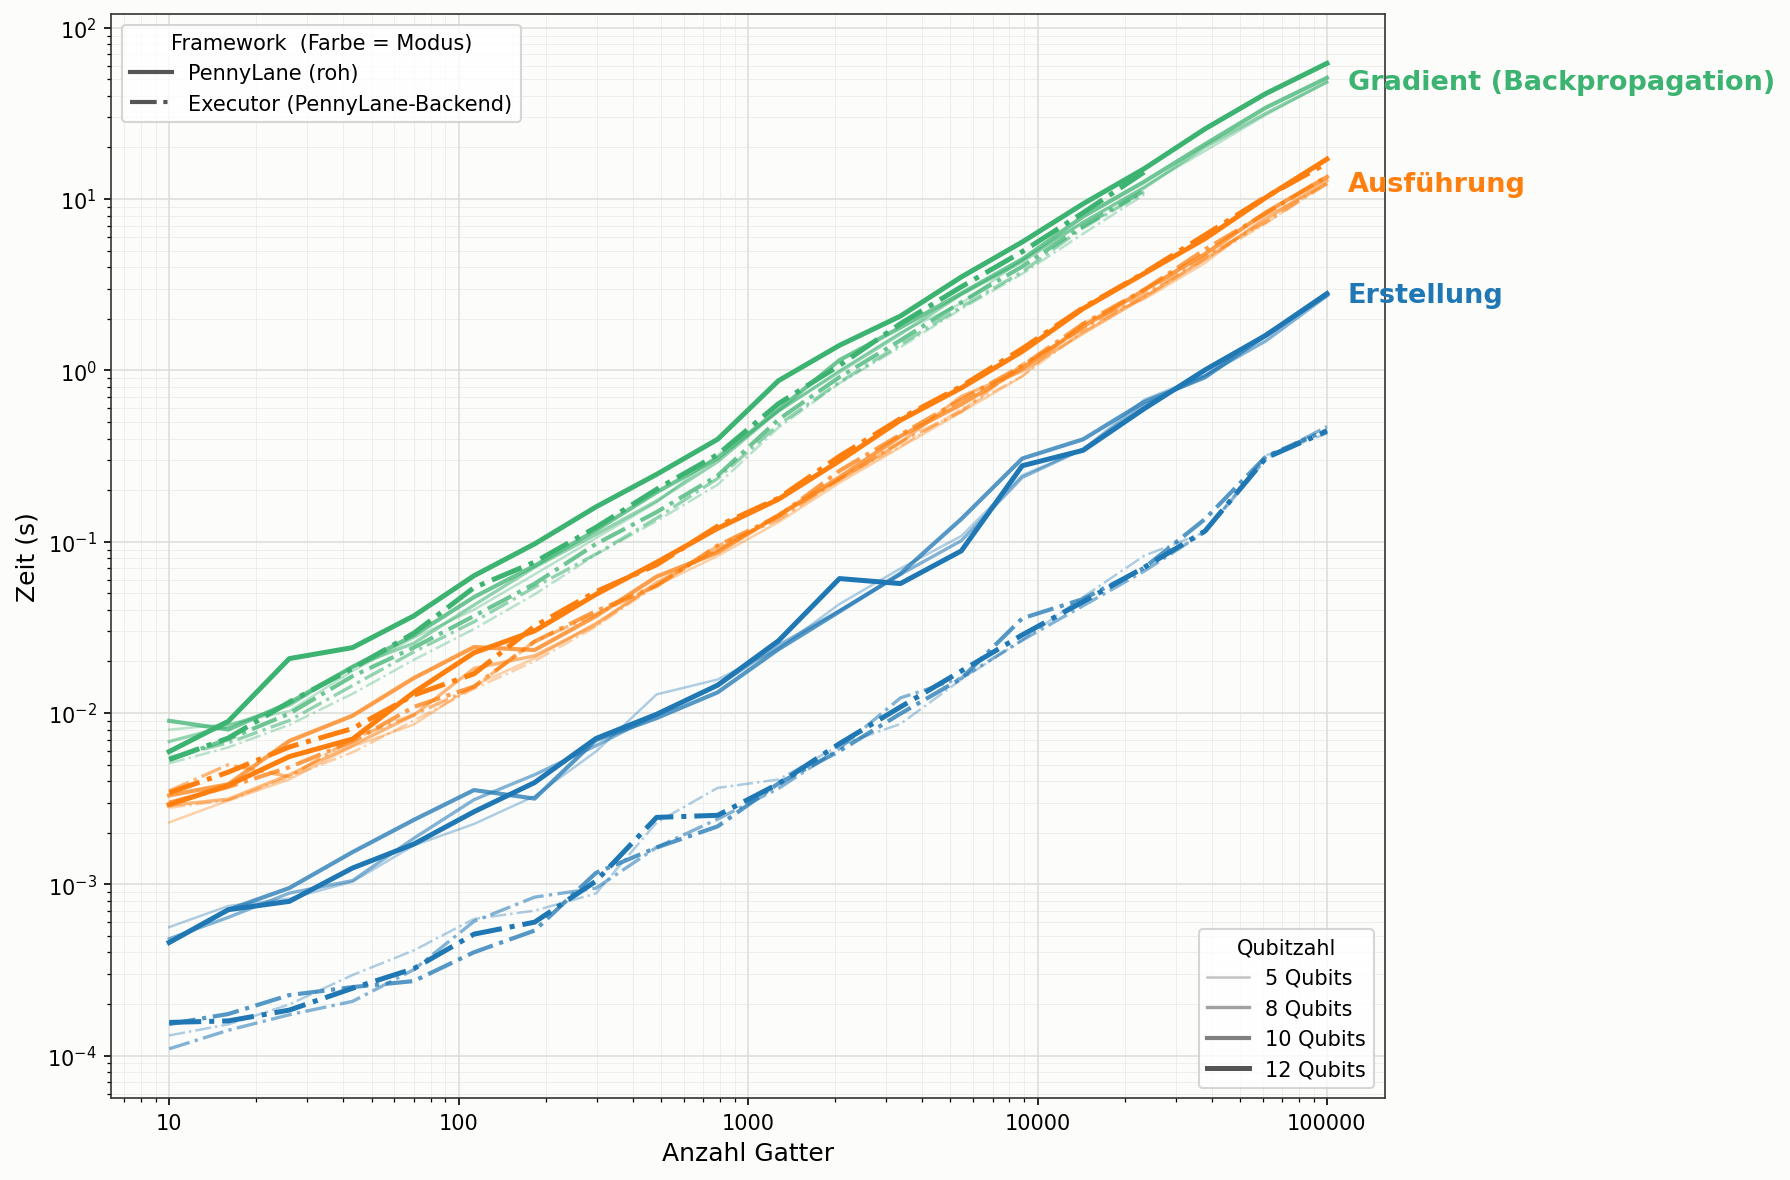
\includegraphics[width=1.1\textwidth]{figures/pennylane_vs_executor_qubits_time_new.png}
    \caption{Laufzeit von nativem \textit{PennyLane} (durchgezogen) und Executor
             mit \textit{PennyLane}-Backend (strichpunktiert)
}
    \label{fig:pennylane-zeit}
\end{figure}

Gemessen wurde über die Qubit-Zahlen 5, 8, 10 und 12 sowie über 20
logarithmisch verteilte Gatterzahlen zwischen 10 und 100\,000, jede Zelle mit
vier Wiederholungen. Abbildung~\ref{fig:pennylane-zeit} zeigt das Ergebnis
doppelt-logarithmisch für alle drei Modi.

Die Qubit-Zahl macht in diesem Bereich nur einen minimalen Unterschied. Die vier
Linien einer Kombination aus Modus und Framework fallen so eng zusammen, dass
sie als ein einziges Band erscheinen. Bei 100\,000 Gattern steigt die native
Laufzeit im Modus \texttt{creation} von $2{,}76$\,s bei 5 Qubits auf
$2{,}80$\,s bei 12 Qubits, im Modus \texttt{execution} von $12{,}1$\,s auf
$17{,}1$\,s. Das ist ein Faktor von $1{,}03$ beziehungsweise $1{,}41$, während
sich der Hilbertraum zwischen beiden Konfigurationen um den Faktor 128
vergrößert. Die Laufzeit wird folglich nicht von der Zustandsvektor-Arithmetik
dominiert, sondern von der pro Gatter anfallenden Python-Arbeit. Nur unter
dieser Voraussetzung wird der Overhead einer zusätzlichen Abstraktionsschicht
überhaupt sichtbar; für deutlich größere Register ist zu erwarten, dass er
relativ zur Simulation verschwindet.

Die Reihen laufen im Modus \texttt{creation} und \texttt{execution} auf beiden
Seiten bis 100\,000 Gatter durch. Im Modus \texttt{gradient} reicht die
Executor-Seite aus Laufzeitgründen nur bis 23\,357 Gatter, die native Seite bis
100\,000. Alle Gradienten-Aussagen beziehen sich daher auf den gemeinsamen
Bereich bis 23\,357 Gatter.

Als Kennzahl dient im Folgenden das geometrische Mittel von
$t_{\mathrm{Executor}}/t_{\mathrm{nativ}}$ über alle Messpunkte ab 1000 Gattern
und alle vier Qubit-Zahlen. Unterhalb von 1000 Gattern liegen die Laufzeiten im
Bereich weniger Millisekunden, wo Einmaleffekte die Verhältnisse verrauschen.

\paragraph*{Erstellung mit erwartbarem Ergebnis}\mbox{}\\
Im Modus \texttt{creation} liegt der Faktor bei $0{,}14$, der Executor ist dort
also rund siebenmal schneller als die native API. Bei 5 Qubits und 100\,000
Gattern stehen $0{,}43$\,s gegen $2{,}76$\,s. Über die vier Qubit-Zahlen ist der
Wert praktisch konstant ($0{,}141$ bis $0{,}146$), und die Steigungen im
Log-Log-Bild sind mit $1{,}07$ bis $1{,}10$ auf beiden Seiten gleich. Es handelt
sich also um einen reinen Vorfaktor und nicht um einen zusätzlichen
Skalierungsterm.

Der Grund liegt darin, dass über die Abstraktionsschicht gar kein vollständiges
Tape entsteht. \verb|ex.transpile_circuit(...)| übersetzt die abstrakte
Gatterliste lediglich in drei parallele Python-Listen mit der
\textit{PennyLane}-Operationsklasse, der Wire-Liste und dem Winkel je Gatter.
Die native Referenz \texttt{qml.\allowbreak workflow.\allowbreak construct\_\allowbreak tape\allowbreak(circuit)()} durchläuft demgegenüber die gesamte Quantenfunktion, instanziiert für jedes Gatter ein
Operationsobjekt, reiht dieses über den Konstruktor in die gerade aktive Queue
ein und setzt daraus ein ausführungsfertiges \texttt{QuantumTape} zusammen.
Tracing, Queuing und Objekterzeugung entfallen beim Executor vollständig.

Diese Zahl ist damit die am wenigsten belastbare der drei und sollte nicht als
Effizienzgewinn gelesen werden, denn beide Seiten leisten hier nicht dieselbe
Arbeit. Das Instanziieren der Operationen holt der Executor bei jeder Ausführung
nach. Der Vorsprung ist keine eingesparte, sondern eine verschobene Arbeit.
Genau deshalb schlägt er im Modus \texttt{execution} nicht mehr durch.

\paragraph*{Ausführung ohne messbaren Overhead}\mbox{}\\
Im Modus \texttt{execution} liegen beide Seiten dicht aufeinander; die
strichpunktierten Executor-Linien liegen innerhalb der Streuung auf den
durchgezogenen nativen Linien. Das geometrische Mittel beträgt $1{,}011$, der
Executor kostet also rund $1$\,\% mehr Laufzeit. Je Qubit-Zahl streut der Wert
zwischen $0{,}99$ und $1{,}03$, in Einzelpunkten zwischen $0{,}82$ und $1{,}12$,
und das Vorzeichen wechselt. Bei 8 und 12 Qubits ist der Executor am rechten
Rand sogar geringfügig schneller ($12{,}31$\,s gegen $12{,}80$\,s
beziehungsweise $16{,}21$\,s gegen $17{,}10$\,s). Ein Overhead von einem Prozent
liegt deutlich unterhalb dessen, was diese Messanordnung auflösen kann; die
belastbare Aussage lautet daher, dass gegenüber \textit{PennyLane} kein
messbarer Overhead entsteht, und nicht, dass er exakt $1{,}1$\,\% beträgt.

Erklärbar ist das über denselben Mechanismus wie bei der Erstellung. Der
Executor spielt bei jedem Aufruf eine vorbereitete Instruktionsliste in einer
Python-Schleife ab, während der native Benchmark die Quantenfunktion erneut
durchläuft und jedes Gatter über die Konstruktoren der Operationsklassen in das
Tape einreiht. Die zusätzliche Ebene des Executors ersetzt hier einen mindestens
ebenso teuren nativen Pfad, statt ihn zu ergänzen.

\paragraph*{Gradientenberechnung mit unerwartetem Ergebnis}\mbox{}\\
Im Modus \texttt{gradient} fällt das Ergebnis unerwartet aus. Das geometrische
Mittel liegt bei $0{,}86$, der Executor ist dort also um 12 bis 15\,\%
\emph{schneller} als die native API, und zwar durchgängig über alle vier
Qubit-Zahlen ($0{,}853$ bis $0{,}878$). Bei 5 Qubits und 23\,357 Gattern stehen
$10{,}60$\,s beim Executor gegen $11{,}83$\,s auf der nativen Seite. Das kann so
nicht stimmen. Der Executor leistet dieselbe Arbeit wie der native Benchmark,
denn Gerät und Schaltkreis sind identisch, und über \verb|diff_method="best"|
rechnet auch er auf \texttt{default.qubit} mit Backpropagation. Zusätzlich
übersetzt er aus der abstrakten Darstellung. Die Abstraktionsschicht müsste
einen Overhead mit sich bringen, kann den nativen Pfad aber nicht unterbieten.

Unabhängig von der Höhe des Faktors ist das Skalierungsverhalten unauffällig.
Beide Seiten wachsen linear in der Gatterzahl, die Steigungen liegen nativ bei
$0{,}99$ bis $1{,}02$ und beim Executor bei $1{,}05$ bis $1{,}07$. Das
bestätigt die Eigenschaft von Backpropagation, dass ein einzelner
Rückwärtsdurchlauf alle Ableitungen liefert und seine Kosten nur von der
Schaltkreisgröße abhängen, nicht von der Parameterzahl; gegenüber der reinen
Ausführung kostet der Gradient lediglich einen konstanten Faktor von etwa 4.
Bemerkenswert ist die kleine, aber über alle vier Qubit-Zahlen gleichgerichtete
Differenz von rund $0{,}05$ im Exponenten. Der Vorsprung des Executors schrumpft
zum rechten Rand hin, von $0{,}86$ im Mittel auf $0{,}89$ bis $0{,}96$ am
letzten gemeinsamen Messpunkt. Der Effekt ist also nicht konstant, sondern
zehrt sich mit wachsender Schaltkreisgröße auf.

\paragraph*{Diskussion des Gradienten-Ergebnisses}\mbox{}\\
Als Ursache für den Wert $0{,}86$ kommt in erster Linie die Laufzeitumgebung in
Betracht, denn die Executor-Gradientenreihe stammt nicht aus demselben Lauf wie
die übrigen Messungen. Der Docker-Container, in dem die Benchmarks ausgeführt
werden, wurde während des ursprünglichen Laufs abgebrochen; die Gradientenreihe
des Executors wurde deshalb am 31.\,07.\,2026 als eigener Lauf nachgezogen,
während alle übrigen Reihen beider Seiten vom 27.\,07.\,2026 stammen. Zwischen
beiden Zeitpunkten wurde das Container-Image neu gebaut, und dabei änderte sich
die \textit{PennyLane}-Version. In der Abhängigkeitsliste war \textit{PennyLane}
zunächst ohne Versionsangabe geführt, sodass die nativen Reihen gegen die zum
Build-Zeitpunkt jeweils neueste Version liefen; für den nachgezogenen
Gradientenlauf des Executors war die Abhängigkeit dagegen auf
\textit{PennyLane}~0.42.3 festgeschrieben. Die beiden Seiten des
Gradienten-Vergleichs wurden also nicht gegen dieselbe Bibliotheksversion
gemessen. Da ein wesentlicher Teil der gemessenen Zeit in \textit{PennyLane}s
eigener Python-Schicht anfällt, also in Tracing, Queuing und Preprocessing des
Tapes, schlagen sich Änderungen an dieser Schicht unmittelbar in der Laufzeit
nieder, und zwar nur auf einer der beiden Seiten des Vergleichs. Wie groß dieser
Beitrag ist, lässt sich nachträglich nicht quantifizieren, da für den früheren
Lauf nur die Abhängigkeit ohne Versionsangabe dokumentiert ist und nicht die
tatsächlich installierte Version.

\newpage
\section{Ergebnisse des Vergleichs von Qiskit und Executor}
\label{sec:ergebnisse-qiskit}

\begin{figure}[H]
    \centering
    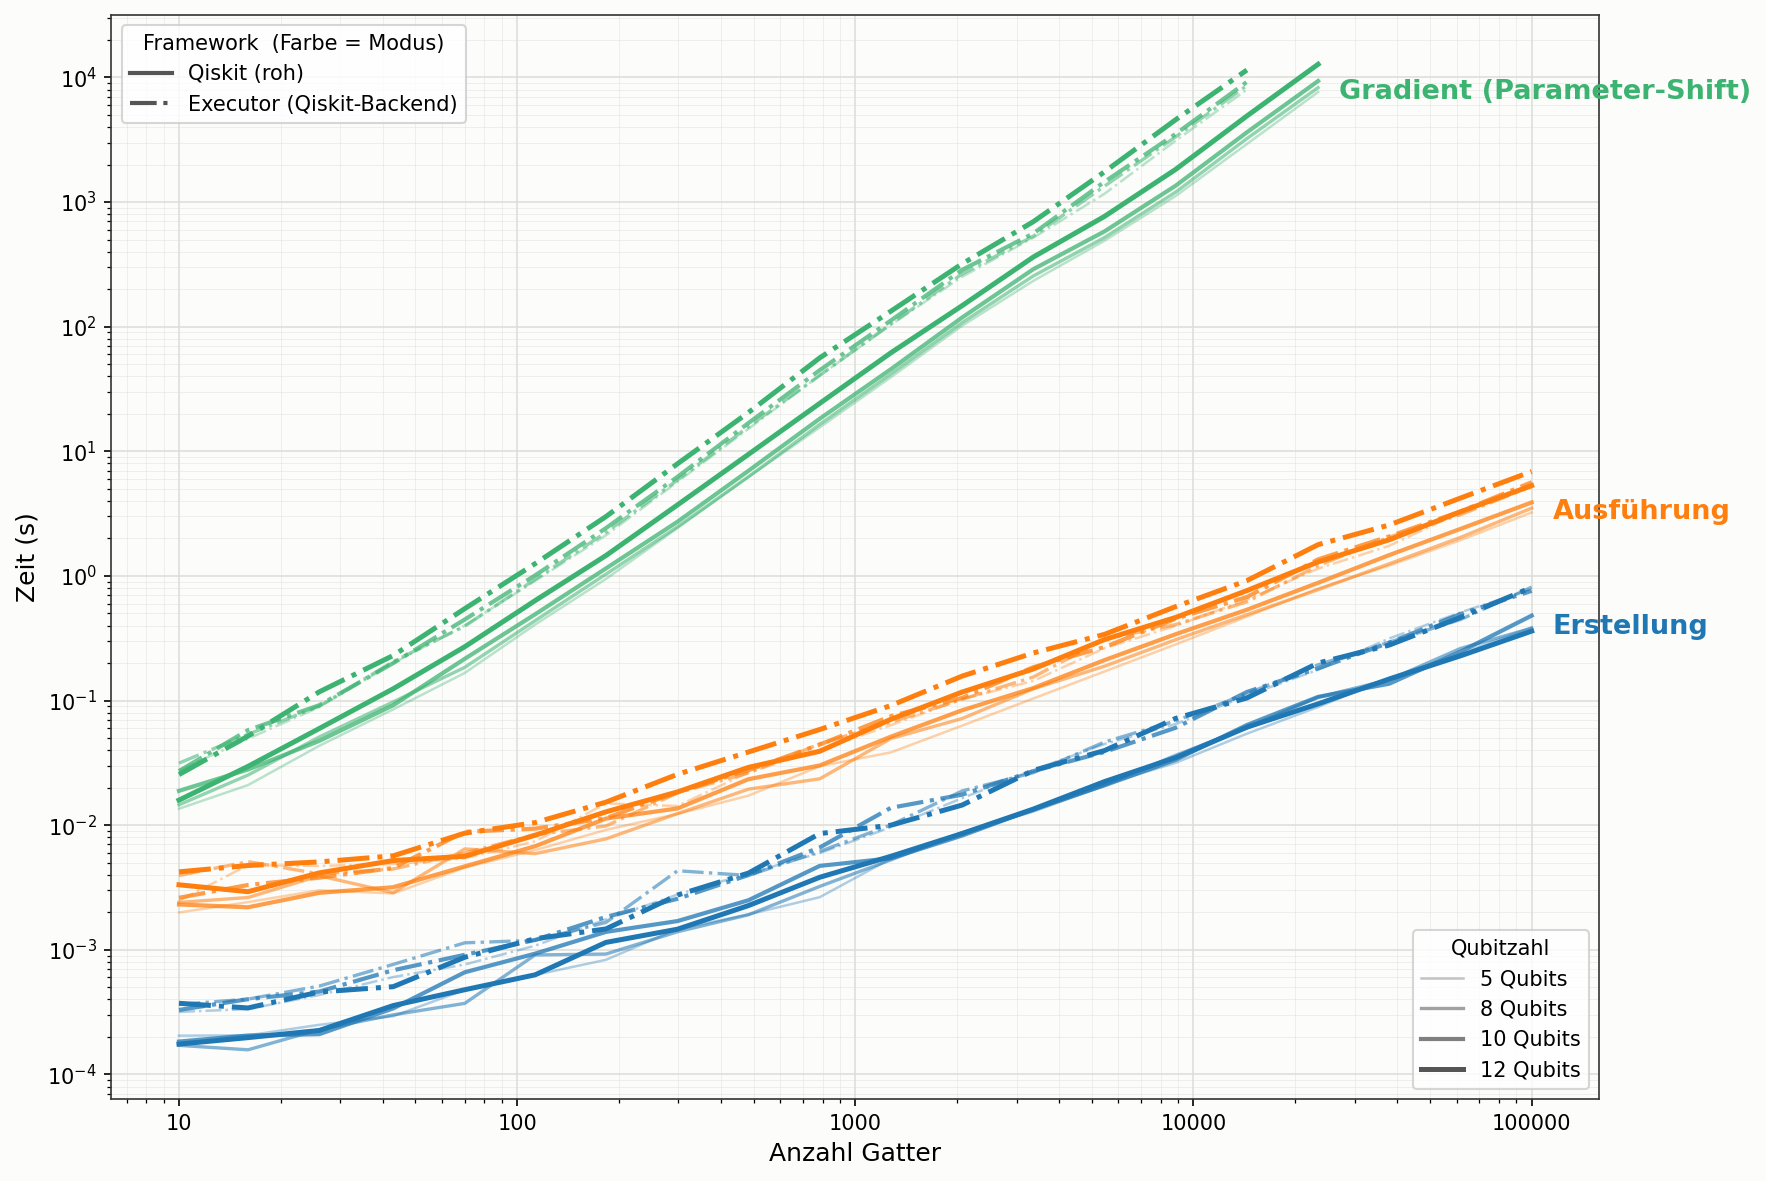
\includegraphics[width=1.1\textwidth]{figures/qiskit_vs_executor_qubits_time.png}
    \caption{Laufzeit von nativem \textit{Qiskit} (durchgezogen) und Executor
             mit \textit{Qiskit}-Backend (strichpunktiert)}
    \label{fig:qiskit-zeit}
\end{figure}

Für das \textit{Qiskit}-Paar gelten dasselbe Messraster und dieselbe Kennzahl
wie oben. Abbildung~\ref{fig:qiskit-zeit} zeigt das Ergebnis in derselben
Auftragung. Das Bild unterscheidet sich in einem Punkt grundlegend von
Abbildung~\ref{fig:pennylane-zeit}. Die strichpunktierten Executor-Linien liegen
in allen drei Modi sichtbar oberhalb der durchgezogenen nativen Linien.
Gegenüber \textit{Qiskit} kostet die Abstraktion also messbar.

Auch hier macht die Qubit-Zahl nur einen minimalen Unterschied, und zwar aus
demselben Grund wie zuvor. Im Modus \texttt{creation} liegen die nativen Zeiten
bei 100\,000 Gattern ohne erkennbaren Trend zwischen $0{,}36$\,s und
$0{,}48$\,s, im Modus \texttt{execution} steigen sie von $3{,}23$\,s bei
5 Qubits auf $5{,}31$\,s bei 12 Qubits. Das ist ein Faktor von $1{,}64$ bei
einem 128-fach größeren Hilbertraum.

Die Gradientenreihe reicht nativ bis 23\,357 Gatter und auf der Executor-Seite
bis 14\,384; die folgenden Gradienten-Aussagen beziehen sich auf den
gemeinsamen Bereich bis 14\,384 Gatter. Der Grund für den früheren Abbruch ist
das Laufzeitbudget, denn eine einzelne Zelle kostet dort bereits mehr als zwei
Stunden.

\paragraph*{Erstellung mit konstantem Faktor 2}\mbox{}\\
Im Modus \texttt{creation} liegt das Verhältnis bei $1{,}97$, die Einzelwerte je
Qubit-Zahl streuen nur zwischen $1{,}93$ und $2{,}02$. Die Steigungen sind mit
$0{,}96$ bis $1{,}02$ auf beiden Seiten praktisch identisch, der Overhead ist
also ein reiner Vorfaktor und kein zusätzlicher Skalierungsterm. Bei 5 Qubits
und 100\,000 Gattern stehen $0{,}79$\,s beim Executor gegen $0{,}39$\,s nativ.

Anders als bei \textit{PennyLane} ist dieser Wert unmittelbar interpretierbar,
denn beide Seiten liefern am Ende dieselbe Datenstruktur, nämlich einen
vollständig befüllten nativen \texttt{QuantumCircuit}. Es wird nichts in eine
spätere Phase verschoben. Der Executor leistet davor zusätzlich die Arbeit der
abstrakten Ebene aus Prüfung jedes Gatters gegen das gemeinsame Vokabular,
Aufbau einer Parameter-Map, Nachschlag der passenden Circuit-Methode und Hashing
für die Memoisierung. Genau diese Zusatzarbeit ist der Faktor 2.

\paragraph*{Ausführung mit Faktor 1,4 und abnehmender Tendenz}\mbox{}\\
Über alle Qubit-Zahlen gemittelt liegt der Overhead bei $1{,}40$. Hier zeigt die
Qubit-Achse als einzige im gesamten Datensatz einen klaren, monotonen Trend. Der
Faktor sinkt von $1{,}51$ bei 5 Qubits über $1{,}44$ und $1{,}38$ auf $1{,}28$
bei 12 Qubits.

Die Erklärung liegt im Nenner und nicht im Zähler. Die absolute Differenz
zwischen beiden Seiten bleibt bei 100\,000 Gattern mit $2{,}07$\,s, $1{,}73$\,s,
$1{,}76$\,s und $1{,}58$\,s über die vier Qubit-Zahlen praktisch konstant,
während die native Laufzeit im selben Schritt von $3{,}23$\,s auf $5{,}31$\,s
wächst. Der Zusatzaufwand des Executors aus Aufbau und Auswertung der
OpTree-Struktur, Deduplizierung und Parameter-Bookkeeping ist reine
Python-Buchhaltung ohne Bezug zur Registergröße. Der relative Overhead wird also
amortisiert, sobald die Simulation teurer wird, und für große Register ist zu
erwarten, dass er weiter gegen 1 läuft.

\paragraph*{Gradientenberechnung mit erwartetem Vorzeichen, aber ohne konstanten
Faktor}\mbox{}\\
Der Gradienten-Modus ist der teuerste Punkt der Paarung mit einem Mittel von
$2{,}40$ und Einzelwerten von $2{,}53$ bei 5 Qubits bis $2{,}22$ bei 12 Qubits.
Anders als bei \textit{PennyLane} fällt das Ergebnis hier in die erwartete
Richtung aus. Der Executor ist langsamer als die native API, so wie es eine
zusätzliche Abstraktionsschicht sein muss. In absoluten Zahlen dauert ein
Gradient bei 5 Qubits und 14\,384 Gattern nativ $2922$\,s und über den Executor
$7985$\,s, was einer Differenz von rund 84 Minuten pro Aufruf entspricht.

Entscheidend ist, dass dieser Faktor als einziger im gesamten Datensatz mit der
Gatterzahl wächst. Über die untere Hälfte des Messbereichs liegt er bei $1{,}91$
bis $2{,}25$, über die obere bei $2{,}23$ bis $2{,}53$ und am letzten
gemeinsamen Messpunkt bei $2{,}34$ bis $2{,}73$. Sichtbar wird das an den
Steigungen im gemeinsamen Bereich, die nativ bei $1{,}74$ bis $1{,}77$ und beim
Executor bei $1{,}78$ bis $1{,}82$ liegen. Die Differenz von rund $0{,}03$ bis
$0{,}04$ im Exponenten ist klein, aber über alle vier Qubit-Zahlen
gleichgerichtet und damit kein Rauschen. Sie passt zu den zwei tiefen
Circuit-Kopien, die der Executor für die Parameter-Shift-Regel je Parameter
anlegt. Jede einzelne kostet $\mathcal{O}(n_{\mathrm{gates}})$ und fällt für
$\mathcal{O}(n_{\mathrm{gates}})$ Parameter an. Zusammen tragen sie damit einen
eigenen quadratischen Term bei, statt den vorhandenen nur zu skalieren.

Dass die gemessenen Exponenten mit etwa $1{,}75$ unterhalb des theoretischen
Werts von 2 liegen, widerspricht dieser Abschätzung nicht. Die Zahl der
Estimator-Läufe wächst exakt linear mit der Gatterzahl, die Kosten eines
einzelnen Laufs steigen im unteren Teil des Messbereichs aber noch unterlinear,
weil dort Fixkosten des Primitivs mitlaufen. Die Steigung nähert sich am rechten
Rand entsprechend an 2 an.

Auf die Einschränkung aus Abschnitt~\ref{sec:ergebnisse-pennylane} ist diese
Paarung nicht angewiesen, denn beide \textit{Qiskit}-Reihen stammen aus
demselben Lauf vom 27.\,07.\,2026 und damit aus demselben Container-Image mit
denselben Bibliotheksversionen. Der Wechsel der \textit{PennyLane}-Version
betrifft sie nicht, und die drei Faktoren sind unabhängig davon interpretierbar.
